\section{Evaluation Report Excluded Data Table}
\label{sec:eval_report_excl_data}

Every Evaluation report obtains a special section 'Excluded Data', where all Evaluation constraints specified in the \nameref{sec:targets} tool of the Flight Deck are listed. 
Also see section \nameref{sec:eval_targets_of_interest_usage} for how to edit this constraints directly from within an Evaluation report.

\begin{figure}[H]
  \hspace*{-2cm}
  \center
    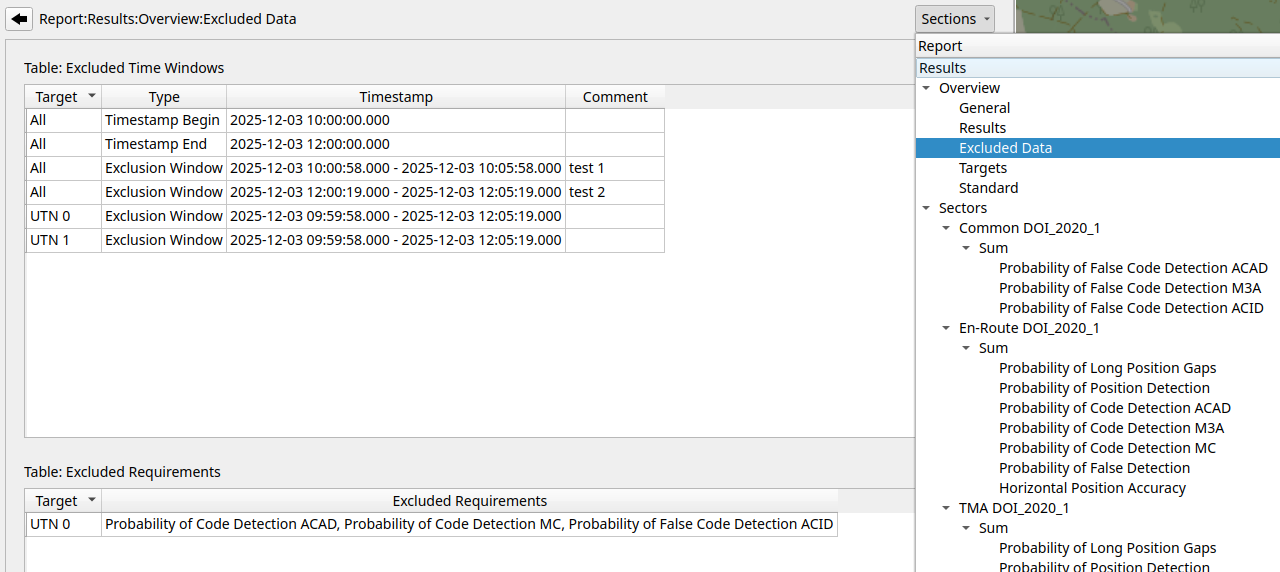
\includegraphics[width=15cm,frame]{figures/eval_excl_data_table.png}
  \caption{Show Evaluation 'Excluded Data' table}
\end{figure}

The first table 'Excluded Time Windows' lists all specified time window based constraints.
First, global constraints are listed, then constraints specified for individual targets. 
See sections \nameref{sec:ui_eval_global_excl_tw} and \nameref{sec:ui_eval_target_excl_tw} 
for how to specify these constraints globally and per target. \\

The table contains the following columns:

\begin{itemize}  
  \item Target: The target the constraint is defined for, either 'All' (globally defined for all targets) or a specific UTN
  \item Type: Constraint type
  \begin{itemize}  
    \item Timestamp Begin: First timestamp to be loaded
    \item Timestamp End: Last timestamp to be loaded
    \item Exclusion Window: Time window excluded from Evaluation
  \end{itemize}
  \item Timestamp: Either a single timestamp or a time window
  \item Comment: Comment optionally added to the constraint
  \end{itemize}
\ \\

The second table 'Excluded Requirements' lists all requirement based constraints specified for individual targets.
See section \nameref{sec:ui_eval_target_excl_req} for how to specify these constraints. \\

The table contains the following columns:

\begin{itemize}  
  \item Target: UTN of the target the constraint is defined for
  \item Excluded Requirements: List of requirements excluded from Evaluation for the specified target
\end{itemize}
\ \\

This section will also be exported to an Evaluation report, so that all constraints 
are documented in a comprehensible way.
